\section{Ecossistema de software acadêmico de análise estática} \label{analise-estatica}

Ao falarmos sobre ecossistema de software acadêmico estamos nos referindo a
qualquer software, de qualquer domínio de aplicação, que tenha sido utilizado
ou produzido durante trabalhos de pesquisa com intuito de publicação na
literatura acadêmica.
%REVER - intuito de apoiar pesquisa que será eventualmente divulgada por meio da  publicação de resultados.

O ecossistema de software acadêmico de análise estática é um recorte deste
conjunto, a princípio, com as mesmas características, atores e modelo de
funcionamento, mas logicamente podendo de apresentar particularidades trazidas
pela natureza do domínio de análise estática e suas ferramentas, soluções e
algoritmos.

\subsection{Análise estática}

A análise estática de código fonte é o primeiro passo para coletar informações
necessárias em diversas atividades de verificação, medição e melhoria da
qualidade de produtos de software \cite{cruz2009code, kirkov2010source}. Ela é
realizada com base no código fonte de um programa ou sistema de software, e a
partir daí descobre problemas e propriedades de sua qualidade estrutural
\cite{chess2007secure}.

Ferramentas de análise estática estão disponíveis há décadas, em especial,
para programadores. A ferramenta Lint \cite{johnson1978lint}, considerada a
primeira ferramenta de análise estática \cite{gosain2015static}, foi criada para
examinar programas escritos em linguagem C e aplicar regras de tipagem mais
estritas do que as regras dos próprios compiladores da linguagem.

Análise estática de código fonte tem como objetivo prover
informações acerca de um programa a partir do seu código fonte sem
necessidade de execução, e sem requerer qualquer outro artefato do programa
além do próprio código.

É um ramo que possui muitas das suas abordagens em comum com os estudos da
área de análise de programas ({\it program analysis}), especialmente na área de
compiladores, onde atua especialmente nas primeiras etapas do processo de compilação.

A análise estática de código fonte é considerada uma atividade meio com
objetivo de suportar uma variedade de tarefas comuns da engenharia de
software; muitas dessas tarefas são substancialmente úteis em atividades de
manutenção. Binkley~\citeonline{binkley2007source} define uma lista dessas
atividades, incluindo:

\begin{multicols}{2}
  \begin{itemize}
    \item Análise de performance
    \item Compreensão de programas
    \item Desenvolvimento baseado em modelos
    \item Detecção de clones
    \item Evolução de software
    \item Garantia de qualidade
    \item Localizaçao de falhas
    \item Manutenção de software
    \item Recuperação arquitetural
    \item Testes
  \end{itemize}
\end{multicols}

Seja em qual atividade for, a análise estática possui importância,
pois ao ser capaz de extrair informações diretamente do
código fonte de um programa, pode auxiliar a responder perguntas necessárias
para as diversas atividades de desenvolvimento e evolução de software. Essa
importância se torna ainda mais aparente diante da ``lei'' da tendência para
execução \cite{harman2010why} que indica que todos os tipos de notação tem a
tendência de se tornar executáveis.

% \subsection{Usos da análise estática de código fonte} \label{usos}

A análise de programas trata, de modo geral, da descoberta de problemas e
fatos sobre programas. Tal análise pode ser realizada sem a necessidade de executar o
programa (análise estática) ou com informações provenientes de sua execução
(análise dinâmica).

A ideia de que programas de computador podem ser utilizados para analisar
código fonte de outros programas tem uma história de mais de 40 anos.  O
programa PFORT \cite{ryder1974pfort} foi projetado para localizar potenciais
problemas na portabilidade de código Fortran; em função da diversidade de
dialetos de Fortran, uma compilação sem erros não indicava que o programa
estava correto segundo os padrões da linguagem \cite{wichmann1995industrial}.

Desde então, ferramentas de análise estática de código fonte têm surgido para
os mais diversos fins -- muitas delas a partir das pesquisas e
desenvolvimentos da área de compiladores.  O {\it parser} utilizado nessas
ferramentas têm funcionalidades análogas aos analisadores usados em
compiladores \cite{anderson2008the}.

O uso de tais ferramentas tem se tornado mais comum no ciclo de desenvolvimento de
software, sendo aplicadas em atividades distintas.
O campo de aplicação destas ferramentas é bastante variado, cobrindo diferentes
objetivos.

\subsection{Software de análise estática}

A variedade de aplicação e a constante evolução da área de análise estática, 
tanto na indústria quando na academia, resulta em  estudos teóricos e práticos, novas ferramentas, modelos e
algoritmos de análise estática. Ferramentas de análise estática têm sido
continuamente desenvolvidas e seu uso se tornado comum no ciclo de desenvolvimento de
software.

Mas apesar da rápida e constante evolução da área, ainda há carência de estudos
avaliando estas ferramentas \cite{li2010comparative}, mesmo com os avanços e com
ferramentas de sucesso, o desenvolvimento de análise estática ainda é conhecido
por ser um processo doloroso \cite{toman2017taming}.

A eficiência, confiabilidade e precisão dessas ferramentas têm sido avaliadas e
alguns estudos mostram inconsistência entre ferramentas diferentes.
Um estudo que comparou duas ferramentas de análise estática para cálculo de métricas,
revelou significantes evidências sobre a inconsistencia entre valores de métricas,
grande diferença nos valores, e discutiu quais problemas e questões levam a estas
diferenças \cite{alemerien2013experimental}.

Análise estática é a técnica mais amplamente utilizada para análise
automatizada de programas devido a sua eficiência, boa cobertura e automação.
Estudos mostram que analise estática tem grande adoção em projetos de software
livre \cite{beller2016analyzing}.
Entretanto,tecnicas de analise estatica amplamente adotadas na comunidade de software,
por exemplo, para localização de bugs e verificação de programas 
ainda sofrem de alto indica de falso-positivos \cite{gosain2015static}.

A crescente atenção que as técnicas de análise estática de código tem
recebido em pesquisas não necessariamente influencia em sua adoção na indústria,
identificando um gap entre pesquisa e indústria \cite{ilyas2016static}.

\subsection{Software acadêmico de análise estática}

Em Ciência da Computação, particularmente em Engenharia de Software, tem-se
notado um aumento constante no número de novos softwares acadêmicos \cite{allen2017engineering},
especialmente em estudos de análise estática, 
uma área com uma longa e respeitável tradição em
pesquisas sobre a criação de novas ferramentas, métodos e algoritmos.

%Na indústria também a adoção de software de análise estática é crescente...

O software acadêmico de análise estática está inserido no contexto similar
a qualquer outro software acadêmico, e o seu ecossistema possui as mesmas
características do ecossistema de software acadêmico, inserido na economia
de reputação científica, Figura \ref{scientific-reputation-diagram} apresenta
o relacionamento entre a prática e pesquisa de software acadêmico.

\begin{figure}[h]
  \center
  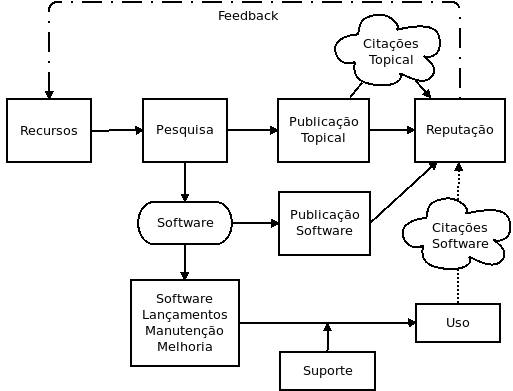
\includegraphics[scale=0.5]{imagens/scientific-reputation-diagram.png}
  \caption{A depiction of the reputation incentives in a mixed science and software academic practice \cite{howison2011scientific}}
  \label{scientific-reputation-diagram}
\end{figure}

%ecossistema de software acadêmico está inserido num contexto de competição

Diferentemente de outras tecnologias, software pode ser copiado e distriduído
essencialmente sem custo, abrindo portas sem precedentes em nível para
compartilhamento e inovação colaborativa \cite{howison2011scientific}, no
entando, estar em algum ponto no contexto de competição da economia de
reputação científica, em alguns pontos, como no mecanismo de crédito acadêmico
às produções ser potencialmente problemático para a colaboração e manutenção
\cite{howison2011scientific}.

No entanto tem se percebido que o ecossistema de software acadêmico tem perdido
oportunidade de colaboração visto que estão inseridos neste contexto ....
competição, muitos softwares utilizados em pesquisas não são mencionados pelos
seus autores causando impacto negativo em sua visibilidade, reconhecimento e
consequentemente ...  \cite{howison2016software}. Esta reflexão tem mostrado,
por exemplo, que muitos estudos em engenharia de software sofrem de
dificuldades de repetição \cite{tang2016worthiness}, e apontam problemas específicos
relacionados à manutenabilidade e a sustentabilidade técnica dos softwares
acadêmicos.

Este cenário, além de desacelerar o progresso geral da Ciência gerando
retrabalho, faz surgir questionamentos sobre as conclusões dessas pesquisas,
especialmente quando grande parte dos pesquisadores não sabem o quão confiável
seus softwares são. Junto com estas questões estão as questões de como
influenciar o ecossistema, incluindo questões de pontos de inflexão que levam
ao uso coalescente, bem como a intervenções políticas diretas incentivando o
uso de componentes específicos.

%%%%%%%%%%%%%%%%%%%%%%%%%%%%%%%%%%%%%%%%%%%%%%%%%%%%%%%%%%%%%%

%While some of these seem relatively unproblematic, such as commercial
%production in fields with immediately valuable applications, others appear
%problematic. In particular we highlighted the potentially pernicious
%implications of the academic credit production system for collaboration and
%maintenance 

%Adicionalmente as relacões entre os atores do ecosistema como um todo
%são de mútuo interesse (mutualismo):

%O relacionamento entre os atores em um ecossistema de software, por outro lado,
%são caracterizados pela alto espectro de relacionamentos simbioticos.

%Dependendo dos atores e suas atividades, dois atores podem ter benefícios
%mútuos (mutualismo), estar em competição direta (competition/antagonism),
%estarem não afetados (neutralism) ou um não afetado enquanto o outro é
%beneficiado (amensalism) ou prejudicado (parasitism) por seu relacionamento

%em pesquisas sobre análise de código, ferramentas de analise estatica tem
%recebido significante mais atencao que outras tecnicas, tecnicas com formal e
%bem definidos processos recebem mais atencao de pesquisa e escrutinio porque
%estudos irao avaliar seu processo e elementos, entretanto, isto nao
%necessariamente significa que tecnica é melhor; The survey concluded that 1)
%the adoption of static code analysis techniques in the industry is influenced
%by the software life cycle model, while software product type and company size
%doesn’t have an influence. 2) The amount of attention a static code analysis
%technique has received in research doesn’t necessarily influence its adoption
%in industry indicating a gap between research and industry 3) company size,
%product type, and life cycle model do influence professionals perception on
%benefits/limitations.  \cite{ilyas2016static}
